%=====================================================================
%  Prueba Técnica — Especialista en Ciencia de Datos
%  Fundación Génesis Empresarial
%  Compilar:  latexmk -pdf informe.tex
%=====================================================================
\documentclass[11pt,a4paper]{article}

\usepackage[T1]{fontenc}
\usepackage[utf8]{inputenc}
\usepackage[spanish,es-nodecimaldot,es-tabla]{babel}

\usepackage{charter}
\usepackage[scaled=0.92]{helvet}
\usepackage{microtype}

\usepackage[a4paper,margin=2.3cm,headheight=14pt]{geometry}
\usepackage{fancyhdr}
\usepackage{titlesec}
\usepackage{enumitem}
\usepackage{setspace}
\onehalfspacing

\usepackage{amsmath}
\usepackage{amssymb}
\usepackage{booktabs}
\usepackage{longtable}
\usepackage{array}
\usepackage{graphicx}
\usepackage{float}
\usepackage[font=small,labelfont=bf]{caption}

\usepackage[most]{tcolorbox}
\usepackage{xcolor}
\definecolor{gprimario}{HTML}{1F4E5F}
\definecolor{gacento}{HTML}{B3261E}
\definecolor{ggris}{HTML}{4A4A4A}
\definecolor{gclaro}{HTML}{EEF3F5}

\usepackage[hidelinks]{hyperref}
\hypersetup{colorlinks=true, linkcolor=gprimario, citecolor=gprimario,
  urlcolor=gprimario, pdftitle={Prueba Técnica - Ciencia de Datos},
  pdfauthor={Julio Vicente}}

\titleformat{\section}{\normalfont\sffamily\Large\bfseries\color{gprimario}}{\thesection}{1em}{}
\titleformat{\subsection}{\normalfont\sffamily\large\bfseries\color{ggris}}{\thesubsection}{1em}{}
\titleformat{\subsubsection}{\normalfont\sffamily\normalsize\bfseries\color{ggris}}{\thesubsubsection}{1em}{}

\pagestyle{fancy}
\fancyhf{}
\renewcommand{\headrulewidth}{0.4pt}
\fancyhead[L]{\footnotesize\sffamily Prueba Técnica · Ciencia de Datos}
\fancyhead[R]{\footnotesize\sffamily Fundación Génesis Empresarial}
\fancyfoot[C]{\footnotesize\sffamily\thepage}

\newtcolorbox{hallazgo}[1][]{enhanced, colback=gclaro, colframe=gprimario,
  boxrule=0.8pt, arc=2pt, left=8pt, right=8pt, top=6pt, bottom=6pt,
  fonttitle=\sffamily\bfseries, title={#1}}
\newtcolorbox{nota}{enhanced, colback=white, colframe=ggris, boxrule=0.5pt,
  arc=1pt, left=8pt, right=8pt, top=5pt, bottom=5pt}
\newtcolorbox{alerta}[1][]{enhanced, colback=white, colframe=gacento,
  boxrule=0.9pt, arc=1pt, left=8pt, right=8pt, top=6pt, bottom=6pt,
  fonttitle=\sffamily\bfseries, title={#1}}

\newcommand{\inciso}[1]{%
  \vspace{0.2em}\noindent\textcolor{gacento}{\sffamily\bfseries\small
  $\blacktriangleright$~Responde al inciso #1}\vspace{0.3em}\par}

\newcommand{\T}[1]{\input{outputs/tex/#1.tex}}
\newcommand{\AUCROC}{0.940}
\newcommand{\AUCPR}{0.835}
\newcommand{\KSmodelo}{0.737}
\newcommand{\BrierSC}{0.0877}
\newcommand{\BrierCal}{0.0869}
\newcommand{\CapturaDiez}{35}
\newcommand{\CapturaVeinte}{62}
\newcommand{\CapturaTreinta}{82}
\newcommand{\LiftUno}{3.51}
\newcommand{\AUCSinSaldo}{0.850}
\newcommand{\AUCROCcv}{0.944}
\newcommand{\NModelable}{66\,038}
\newcommand{\PrevalenciaKdos}{26.1}
\newcommand{\TasaKuno}{49.6}
\newcommand{\ProbMedia}{34.4}
\newcommand{\FugasEsperadas}{3\,442}
\newcommand{\NCampana}{4\,957}
\newcommand{\SaldoTotal}{57.2}
\newcommand{\SaldoAlto}{2.6}
\newcommand{\NTickets}{9\,981}
\newcommand{\NReglas}{352}
\newcommand{\NCanastas}{14}
\newcommand{\LiftMax}{36.4}
\newcommand{\ProdTop}{Coffee Eclair}
\newcommand{\SoporteTop}{10.9}
\newcommand{\ItemsTicket}{3.56}

%=====================================================================
\begin{document}

%---------------------------------------------------------- PORTADA
\begin{titlepage}
\centering
\vspace*{2.2cm}

{\sffamily\Huge\bfseries\color{gprimario}
Modelo de predicción de fuga\\[0.25em]
y segmentación de clientes\par}

\vspace{0.9cm}
{\sffamily\large\color{ggris}
Prueba técnica --- Especialista en Ciencia de Datos\par}

\vspace{0.4cm}
{\sffamily\large Fundación Génesis Empresarial\par}

\vspace{2.2cm}
\rule{0.5\textwidth}{0.8pt}

\vspace{1.1cm}
{\large\textbf{Julio Vicente}\par}
\vspace{0.3em}
{\small\texttt{joulefvicente@gmail.com}\par}

\vspace{1.8cm}
\begin{minipage}{0.82\textwidth}\centering\small\color{ggris}
El modelo captura el \CapturaVeinte\% de las fugas contactando al 20\% de la
cartera. La probabilidad entregada está calibrada: en el decil de mayor riesgo
predice 93\% y se retira el 92\%.
\end{minipage}

\vfill
{\small \today\par}
\end{titlepage}

%---------------------------------------------------- MAPA DE RESPUESTAS
\section*{Mapa de respuestas}
\addcontentsline{toc}{section}{Mapa de respuestas}

\noindent Ubicación de la respuesta a cada inciso del enunciado:

\vspace{0.6em}
\noindent\begin{tabular}{@{}p{0.08\textwidth}p{0.62\textwidth}p{0.24\textwidth}@{}}
\toprule
\textbf{Inciso} & \textbf{Requerimiento} & \textbf{Sección} \\
\midrule
1.a & Algoritmos utilizados en el modelo de fuga & \S\ref{sec:algoritmos} \\
1.b & Algoritmo de la probabilidad y justificación & \S\ref{sec:calibracion} \\
1.c & Variables de mayor impacto & \S\ref{sec:shap} \\
1.d & \% de probabilidad de fuga por cliente & \S\ref{sec:probabilidades} + XLSX \\
1.e & Clientes recomendados para campaña & \S\ref{sec:campana} + XLSX \\
1.f & Segmentación, dashboard y patrones & \S\ref{sec:segmentacion} y \S\ref{sec:tablero} \\
2.a & Reglas de asociación & \S\ref{sec:reglas} \\
2.b & Justificación de las reglas elegidas & \S\ref{sec:criterio} \\
2.c & Uso recomendado de los resultados & \S\ref{sec:usobakery} \\
3   & Tablero de visualización & \S\ref{sec:tablero} \\
\bottomrule
\end{tabular}

\vspace{1.2em}
\begin{nota}
\small\textbf{Archivos que acompañan a este informe:}
\begin{itemize}[leftmargin=1.2em,nosep]
\item \texttt{Genesis\_Churn\_Prediccion\_Julio\_Vicente.xlsx} --- los 10\,000 clientes
      con su probabilidad, decil, segmento y recomendación de campaña (incisos 1.d y 1.e).
\item \texttt{Genesis\_Segmentacion\_Julio\_Vicente.xlsx} --- perfiles de segmento y
      asignación por cliente (inciso 1.f).
\item \texttt{Genesis\_Reglas\_Asociacion\_Julio\_Vicente.xlsx} --- reglas de asociación (inciso 2).
\item \texttt{Genesis\_Auditoria\_Datos\_Julio\_Vicente.xlsx} --- evidencia de la auditoría de datos.
\item \texttt{Tablero\_Cartera\_Riesgo\_Julio\_Vicente.html} --- tablero interactivo de
      cinco páginas, autónomo (inciso 3). Descrito en \S\ref{sec:tablero}.
\end{itemize}
El detalle por cliente no se imprime en este documento: aquí van los resultados
agregados y la justificación metodológica.
\end{nota}

\clearpage
\tableofcontents
\clearpage

%==================================================================== 1
\section{Resumen ejecutivo}

De los 10\,000 clientes activos, el modelo espera que se retiren
\textbf{\FugasEsperadas} (\ProbMedia\% de la cartera). Ese riesgo no está
repartido de forma pareja: se concentra, y esa concentración es lo que hace
accionable el modelo.

\begin{hallazgo}[Los tres números que importan]
\begin{enumerate}[leftmargin=*,nosep]
  \item \textbf{Contactando al 20\% de los clientes de mayor riesgo se alcanza al
        \CapturaVeinte\% de quienes se van a retirar.} Al 30\%, se alcanza al
        \CapturaTreinta\%. El decil más riesgoso concentra \LiftUno~veces más
        fugas que un grupo elegido al azar.
  \item \textbf{La probabilidad entregada es una probabilidad real, no un puntaje.}
        En el conjunto de prueba, el decil superior tiene una probabilidad media
        predicha de 93.3\% y una tasa observada de 92.2\%. La correspondencia se
        mantiene decil a decil (tabla~\ref{tab:calib}).
  \item \textbf{Se recomienda contactar a \NCampana\ clientes} bajo el supuesto
        base de 20\% de efectividad de campaña, con un retorno esperado de
        3.6 veces el costo. Si el área comercial sólo puede atender 1\,000
        contactos, la lista priorizada por valor esperado captura el 24\% de
        todas las fugas.
\end{enumerate}
\end{hallazgo}

\subsection*{De qué datos salen estos números}

Se trabajó sobre tres bases: \textbf{78\,829 clientes históricos} con desenlace
conocido --- una fila por cliente, no un panel cliente--mes ---, los
\textbf{10\,000 clientes activos} a los que se aplica el modelo y
\textbf{9\,981 tickets} de la panadería para el ejercicio de canastas. Se
considera \emph{fugado} al cliente cuyo registro figura como \emph{Cliente
Retirado}: cerró su ciclo de crédito sin renovar dentro de la ventana de 30
meses. La prevalencia histórica es de 38.1\%, un desbalance moderado que no
exige remuestreo sintético.

Tres condiciones de los datos determinaron el diseño del trabajo, y conviene
enunciarlas antes que cualquier resultado:

\begin{enumerate}[leftmargin=*]
\item \textbf{La base histórica contiene dos variables que revelan la respuesta.}
      El código de cliente separa retirados y renovados con exactitud perfecta,
      porque el archivo fue ordenado por estado antes de numerarse; y estar en el
      primer crédito implica ser retirado por definición lógica, no por
      comportamiento. Un modelo que las use reporta métricas impecables en
      entrenamiento y produce ruido sobre los 10\,000 activos, cuyos códigos
      fueron renumerados. Ambas se descartaron, y el segmento de primer crédito
      se modela aparte.
\item \textbf{No hay fechas ni comportamiento de pago.} Ninguna base registra
      desembolso, vencimiento, mora ni puntualidad de cuotas. Eso impide una
      validación fuera de tiempo y descarta las variables de tendencia, que en
      cartera de microcrédito suelen ser las más predictivas: el desempeño
      reportado es un piso y no un techo.
\item \textbf{Los montos no son comparables entre las dos bases} --- PSI de 2.74,
      rejillas de valores casi disjuntas. El modelo se apoya por eso en el
      \emph{ratio saldo/capital}, invariante a la escala del monto, y no en el
      monto absoluto.
\end{enumerate}

\noindent La validación se hizo sobre \textbf{tres bloques disjuntos}
(entrenamiento 60\%, calibración 20\%, prueba 20\%) agrupados por vector de
atributos, de modo que filas idénticas nunca queden a la vez en entrenamiento y
prueba; la semilla es fija y el bloque de prueba no se tocó hasta producir las
cifras de este informe. La evidencia numérica de las tres condiciones anteriores
y el detalle del esquema están en \S\ref{sec:datos}.

\subsection*{Dónde está el dinero, y dónde está el riesgo}

No son el mismo lugar, y conviene decirlo con claridad: los clientes con mayor
probabilidad de fuga son los de \emph{menor} saldo, porque el saldo bajo es
justamente la señal de que el crédito está por terminar. El segmento de riesgo
alto representa \$\SaldoAlto~millones de saldo vigente sobre un total de
\$\SaldoTotal~millones. Por eso la campaña no se prioriza por saldo actual sino
por el \textbf{margen del ciclo de crédito que se perdería} si el cliente no
renueva (\S\ref{sec:campana}).

%==================================================================== 2
\section{Datos, auditoría y validación}
\label{sec:datos}

Esta sección aporta la evidencia de lo que el resumen enuncia. Es el núcleo
metodológico del trabajo: sin las dos correcciones que aquí se documentan, las
métricas del modelo serían impecables y sus predicciones, inservibles.

\subsection{Las tres bases}

\begin{description}[leftmargin=1.4em,style=nextline,nosep]
\item[Base de Datos Modelo] 78\,829 registros, 14 columnas, una fila por cliente:
      los códigos de cliente son únicos y el código de préstamo es exactamente
      diez veces el código de cliente. No es un panel cliente--mes, pese a que el
      enunciado menciona 30 meses de comportamiento.
\item[Base de Datos Predicción] 10\,000 clientes activos, las mismas 13 variables
      explicativas más las dos columnas a completar (\emph{Probabilidad Fuga} y
      \emph{Predicción}).
\item[Bakery] 9\,981 tickets $\times$ 50 productos, ya en formato de matriz
      transaccional binaria.
\end{description}

\begin{nota}
\small \textbf{Unidad monetaria.} Las bases no declaran la unidad de los importes.
Tratándose de una empresa colombiana, todas las cifras de dinero de este informe
se expresan en \textbf{pesos colombianos (COP)} y se presentan en la escala
original del archivo, sin conversión. Los supuestos económicos de la campaña
(\S\ref{sec:campana}) se fijaron en esa misma escala, de modo que la decisión de
a quién contactar no depende de la unidad elegida.
\end{nota}

\subsection{Auditoría de variables}
\label{sec:auditoria}

Una variable tiene fuga de información cuando sólo pudo conocerse \emph{después}
o \emph{a causa} de que el cliente se fuera; usarla produce un modelo que parece
excelente y no sirve. El diagnóstico se hizo calculando el AUC univariado de cada
variable contra el objetivo, y dos resultados obligaron a intervenir: el
identificador de cliente y el indicador de primer crédito, ya enunciados en el
resumen. \textbf{Su evidencia numérica completa está en el anexo~\ref{ap:evidencia}},
junto con la deriva de montos entre bases y la verificación de que el saldo sí es
comparable. La tabla siguiente recoge la decisión adoptada sobre cada variable.

\begin{table}[H]\centering\small
\caption{Decisión adoptada sobre cada variable y su justificación.}
\T{auditoria}
\end{table}

\noindent Se corrigieron además dos defectos de calidad: \texttt{TIPO DE CREDITO}
presentaba 12 niveles aparentes que se reducen a 8 tras normalizar espacios en
blanco y mayúsculas (los valores \texttt{`C'} y \texttt{`C~~~'} figuraban como
categorías distintas), y un registro tenía el sexo en blanco.

\subsection{Esquema de validación}
\label{sec:validacion}

\begin{description}[leftmargin=1.4em,style=nextline,nosep]
\item[Tres bloques disjuntos] Entrenamiento 60\%, calibración 20\%, prueba 20\%.
      El bloque de calibración es independiente del de entrenamiento, y el de
      prueba no se tocó hasta producir las cifras finales de este informe.
\item[Agrupación por vector de atributos] 7\,803 filas tienen atributos idénticos
      a otra fila. Con particiones aleatorias simples caerían a la vez en
      entrenamiento y prueba e inflarían artificialmente las métricas; las
      particiones se construyeron agrupando por el vector de atributos.
\item[Validación cruzada] Cinco particiones estratificadas y agrupadas, para
      comparar la escalera de modelos con predicciones fuera de partición.
\item[Reproducibilidad] Semilla fija (42) en todos los procesos.
\end{description}

\noindent Como no hay fechas, no es posible una validación fuera de tiempo, que
sería el esquema correcto para replicar las condiciones de aplicación; el diseño
anterior es su sustituto. Se deja constancia, además, de que 587 grupos de
atributos idénticos presentan ambos desenlaces: ese es el ruido irreducible del
problema y fija un techo al desempeño alcanzable con las variables disponibles.

%==================================================================== 3
\section{Modelo de predicción de fuga}

\subsection{Algoritmos evaluados}
\label{sec:algoritmos}
\inciso{1.a}

Se evaluó una escalera completa de modelos, de menor a mayor complejidad, y se
reporta entera: presentar únicamente el ganador oculta si la complejidad
adicional estaba justificada.

\begin{table}[H]\centering\small
\caption{Escalera de modelos. Métricas fuera de partición sobre el bloque de
entrenamiento, salvo la regla de negocio.}
\label{tab:escalera}
\T{escalera}
\end{table}

\begin{description}[leftmargin=1.4em,style=nextline,nosep]
\item[Nivel 0 --- Regla de negocio] ``Está en riesgo si ya amortizó más del 85\%
      de su crédito o si está en etapa M2/M3''. Es la línea base que la gerencia
      ya entiende, y sirve para medir cuánto aporta realmente el modelo.
\item[Nivel 1 --- Regresión logística] Referencia obligada en riesgo crediticio
      por su interpretabilidad. Con codificación \emph{one-hot} y estandarización
      dentro de un \emph{pipeline} ajustado sólo con datos de entrenamiento.
\item[Nivel 2 --- Random Forest] Referencia no lineal.
\item[Nivel 3 --- LightGBM] Modelo seleccionado. Maneja las categóricas de alta
      cardinalidad de forma nativa (138 agencias, 40 subproductos) sin expandir la
      matriz.
\item[Nivel 4 --- Ensamble] Promedio de rangos de los tres anteriores. No mejoró
      al LightGBM en solitario, de modo que se descartó: no se añade complejidad
      que no paga.
\end{description}

\noindent Se incluye además una \textbf{prueba de robustez} (fila 3b): el mismo
LightGBM entrenado sin ninguna variable derivada del saldo alcanza AUC-ROC de
\AUCSinSaldo, frente a \AUCROCcv\ del modelo completo medido sobre el mismo
esquema de validación cruzada. Es decir, el modelo conserva capacidad predictiva
sustancial incluso si se sospechara del saldo, lo que acota el riesgo de que el
resultado dependa de una sola familia de variables.

\subsection{Modelo seleccionado y calibración de probabilidades}
\label{sec:calibracion}
\inciso{1.b}

\begin{nota}
\textbf{Respuesta directa:} se utilizó \textbf{LightGBM} (\emph{gradient boosting}
sobre árboles) para ordenar el riesgo, y \textbf{regresión isotónica} ajustada
sobre un conjunto de calibración independiente para convertir ese ordenamiento en
una probabilidad interpretable como porcentaje. La verificación se hizo con curva
de confiabilidad y \emph{Brier score}.
\end{nota}

\noindent La distinción importa porque el inciso 1.d pide un \emph{porcentaje} de
probabilidad, no un puntaje. Un modelo puede ordenar perfectamente a los clientes
y aun así entregar números que no signifiquen nada como probabilidad. Por eso se
separan las dos tareas:

\begin{enumerate}[leftmargin=*,nosep]
\item \textbf{Ordenar} --- LightGBM, elegido por desempeño en la tabla~\ref{tab:escalera}.
\item \textbf{Calibrar} --- regresión isotónica, ajustada exclusivamente sobre el
      bloque de calibración, nunca sobre los datos de entrenamiento ni sobre los
      de prueba.
\end{enumerate}

\noindent El \emph{Brier score} sobre el conjunto de prueba pasa de \BrierSC\ sin
calibrar a \BrierCal\ tras la calibración isotónica. Se probó también el método de
Platt, que resultó peor (0.0917). Conviene señalar con honestidad que
\textbf{la mejora por calibrar fue marginal}: el LightGBM ya salía prácticamente
calibrado. Se conserva la isotónica porque el inciso pide explícitamente un
porcentaje y la garantía adicional no tiene costo relevante.

\subsubsection*{Sobre el desbalance}

No se aplicó SMOTE ni submuestreo. Con 38\% de prevalencia el desbalance es
moderado, y ambas técnicas \textbf{destruyen la calibración de las
probabilidades}, que es precisamente lo que el inciso 1.d requiere. Se usó
ponderación de clases donde correspondía, y se evitó la métrica de exactitud
(\emph{accuracy}) en todo el ejercicio.

\subsection{Desempeño}

\begin{table}[H]\centering\small
\caption{Probabilidad predicha frente a tasa real observada, por decil de riesgo,
sobre el 20\% de datos reservados. Es la evidencia central de que la probabilidad
entregada es utilizable como porcentaje.}
\label{tab:calib}
\T{calibracion}
\end{table}

\noindent Las dos columnas centrales coinciden decil a decil. Cuando el modelo
dice 93\%, se retiran 92 de cada 100; cuando dice 28\%, se retiran 30 de cada 100.
Las métricas globales sobre el mismo conjunto son: AUC-ROC \AUCROC, AUC-PR
\AUCPR\ y KS \KSmodelo.

\begin{figure}[H]\centering
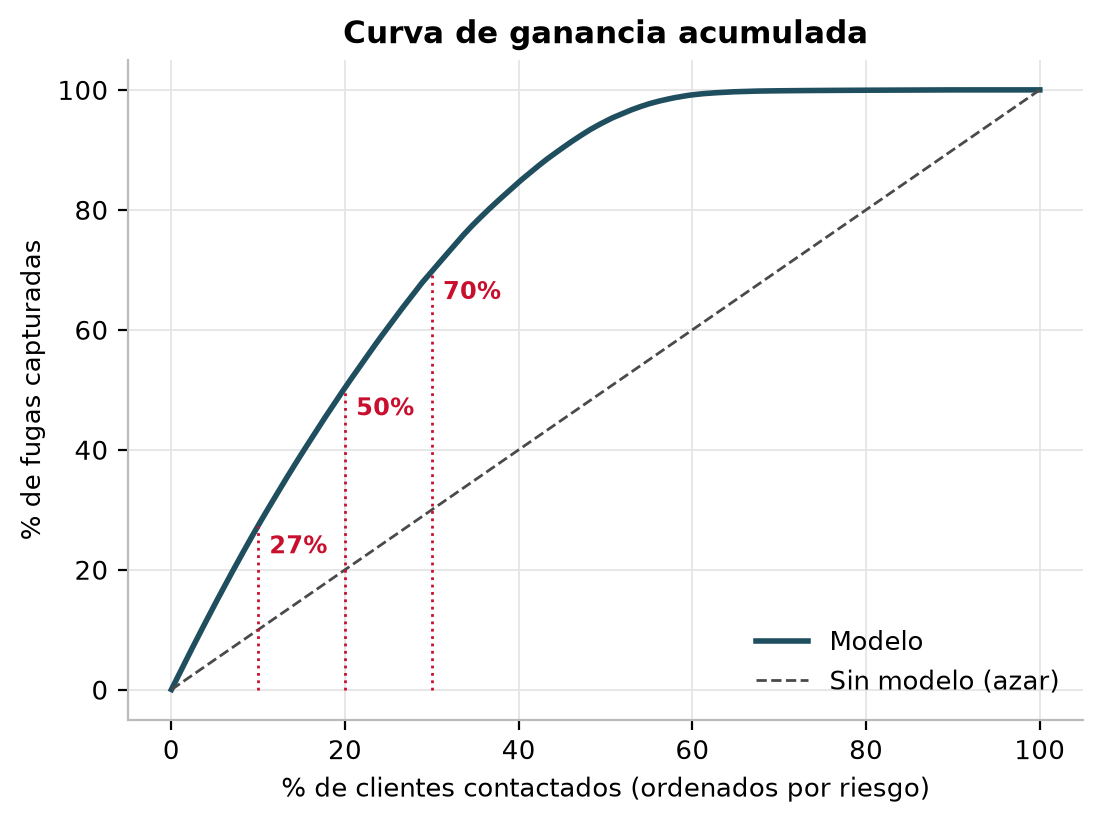
\includegraphics[width=0.62\textwidth]{outputs/figuras/07_curva_ganancia.png}
\caption{Curva de ganancia acumulada sobre la cartera activa. Contactando al 20\%
de mayor riesgo se cubre el \CapturaVeinte\% de las fugas esperadas.}
\end{figure}

\subsection{Variables de mayor impacto}
\label{sec:shap}
\inciso{1.c}

La importancia se midió con \textbf{SHAP} y no con la importancia por ganancia de
los árboles, que está sesgada hacia variables de alta cardinalidad y no indica el
sentido del efecto.

\begin{table}[H]\centering\small
\caption{Variables ordenadas por su peso relativo en la decisión del modelo.}
\T{shap}
\end{table}

\begin{figure}[H]\centering
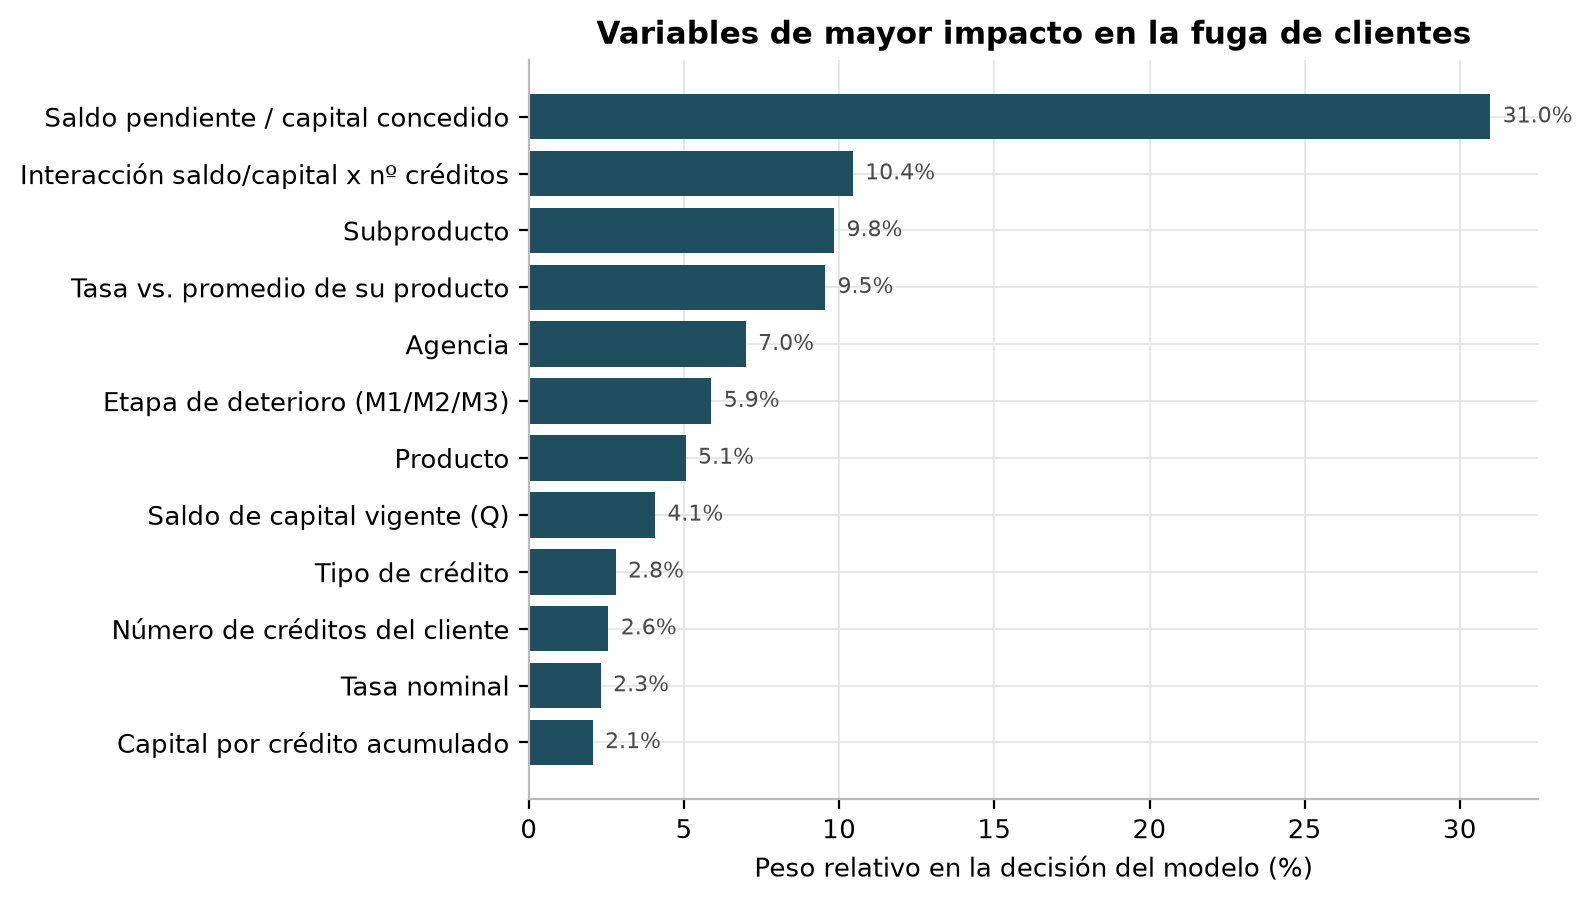
\includegraphics[width=0.92\textwidth]{outputs/figuras/06_shap_barras.png}
\caption{Peso relativo de cada variable.}
\end{figure}

\subsubsection*{Traducción al lenguaje del negocio}

\begin{description}[leftmargin=1.4em,style=nextline,nosep]
\item[1. Qué tan avanzado va el cliente en el pago de su crédito (31\% del peso)]
      Es, con diferencia, la señal dominante. Un cliente que ya amortizó más del
      90\% de su crédito y no ha vuelto a solicitar está en la puerta de salida:
      en ese tramo la tasa de fuga histórica es del 81\%. Un cliente con un
      desembolso reciente y más del 60\% del capital pendiente prácticamente no
      se va: su tasa es del 1\% al 5\%. \textbf{La fuga en microcrédito no ocurre
      en cualquier momento: ocurre en la ventana de renovación.}
\item[2. La interacción entre el avance del crédito y la antigüedad (10\%)]
      El mismo nivel de amortización significa cosas distintas según la
      trayectoria del cliente. Un cliente en su segundo crédito con el 90\%
      pagado se retira en el 81\% de los casos; uno en su noveno crédito, en el
      12\%. \textbf{La lealtad acumulada amortigua el riesgo de la ventana de
      renovación.}
\item[3. Subproducto y tasa relativa a su producto (19\% combinado)]
      La tasa que se le cobra al cliente \emph{comparada con la de sus pares del
      mismo producto} pesa más que la tasa en términos absolutos. Es un hallazgo
      accionable: sugiere sensibilidad al precio relativo, no al precio.
\item[4. Agencia (7\%)] Hay diferencias sistemáticas de retención entre agencias
      que las variables del cliente no explican. Apunta a prácticas comerciales
      locales y merece revisión operativa.
\item[5. Etapa de deterioro (6\%)] Los clientes en M3 se retiran en el 98\% de los
      casos. Es una señal potente, pero llega tarde: cuando aparece, la retención
      comercial ya no es el instrumento adecuado.
\end{description}

\subsubsection*{Contraste y estabilidad}

El coeficiente del ratio saldo/capital en la regresión logística es $-3.10$
(razón de momios 0.045), el segundo de mayor magnitud del modelo lineal. Los dos
enfoques, uno lineal y otro basado en árboles, coinciden en señalar la misma
variable como dominante y en la misma dirección, lo que refuerza la lectura.

El ranking se recalculó en cinco particiones independientes: las ocho primeras
variables mantienen su posición con desviación estándar de 0 a 1 puesto. La
jerarquía no es un artefacto de una partición concreta.

%==================================================================== 4
\section{Aplicación a los clientes activos}

\subsection{Tratamiento del segmento de primer crédito}
\label{sec:primercredito}

Antes de presentar las probabilidades hay que resolver el problema planteado en
\S\ref{sec:auditoria}: en el histórico, el primer crédito determina el objetivo
por definición, de modo que ese subconjunto no aporta información discriminante.
El modelo principal se entrenó, por tanto, sobre los \NModelable\ clientes con
dos o más créditos, donde la tasa de fuga es \PrevalenciaKdos\%.

Para los 1\,873 activos en su primer crédito se separó el problema en dos:

\begin{description}[leftmargin=1.4em,style=nextline,nosep]
\item[El ordenamiento] se toma del modelo entrenado con los demás clientes. Dentro
      del segmento, quien lleva más amortizado y menos saldo sigue siendo el más
      propenso a irse.
\item[El nivel] se estima extrapolando la curva empírica de fuga frente al número
      de créditos. Ajustando una relación logit-lineal sobre los tramos de 2 a 5
      créditos --- donde la extrapolación a 1 es creíble --- se obtiene una tasa
      estimada de \textbf{\TasaKuno\%} para el primer crédito. Se aplica como
      corrección de prior en escala logit, que es una transformación monótona y
      por tanto no altera el ordenamiento.
\end{description}

\noindent La cifra es coherente con lo que se observa en microfinanzas: el primer
ciclo es el de mayor deserción. Y es sustancialmente distinta del 100\% que
arrojaría copiar la tautología del histórico. Se hizo análisis de sensibilidad
sobre este supuesto: variar la tasa entre 30\% y 85\% mueve el número de clientes
de primer crédito entre los 1\,000 de mayor riesgo de 213 a 726, sin alterar la
composición del resto de la lista.

\subsection{Distribución de probabilidades de fuga}
\label{sec:probabilidades}
\inciso{1.d}

El archivo \texttt{Genesis\_Churn\_Prediccion\_Julio\_Vicente.xlsx} contiene la
base original de 10\,000 clientes con las columnas \emph{Probabilidad Fuga}
(0 a 1, cuatro decimales), \emph{prob\_fuga\_pct} (porcentaje), decil de riesgo,
segmento de riesgo, segmento de clustering y recomendación de campaña.

\begin{figure}[H]\centering
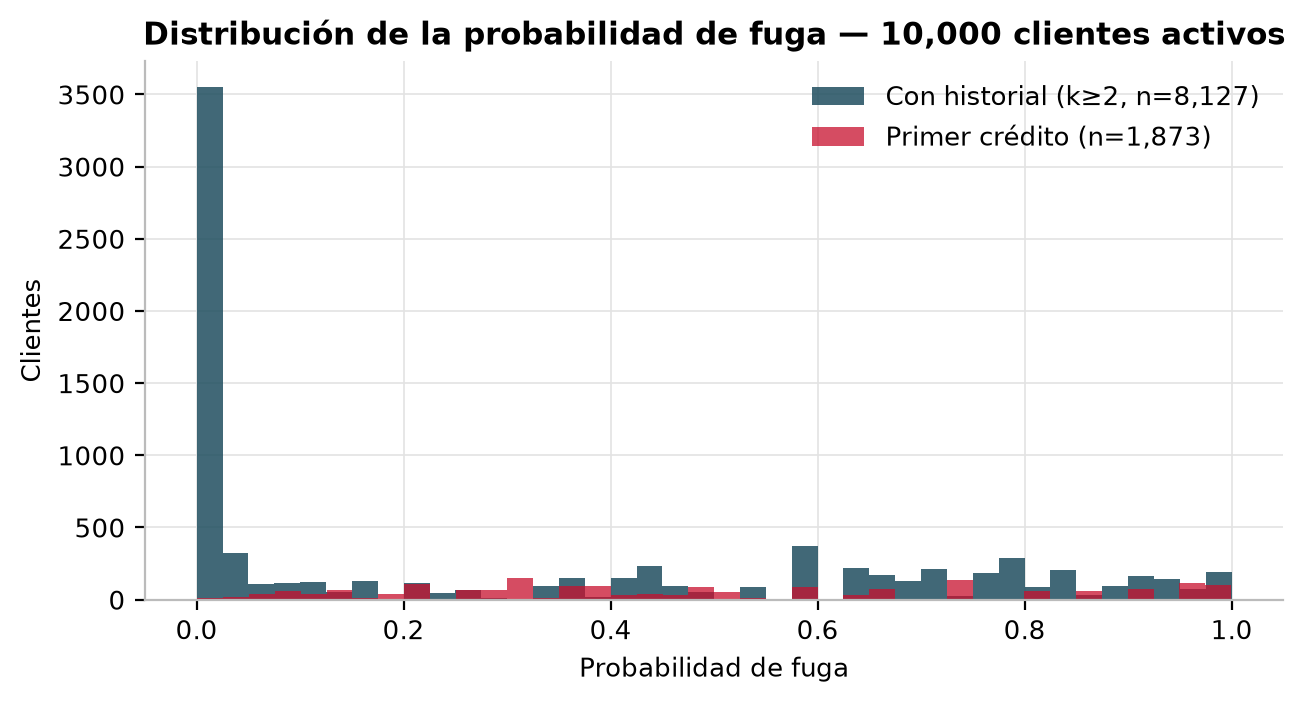
\includegraphics[width=0.82\textwidth]{outputs/figuras/07_distribucion_prob.png}
\caption{Distribución de la probabilidad de fuga. La cartera se separa en dos
poblaciones nítidas; hay poca zona intermedia.}
\end{figure}

\begin{table}[H]\centering\small
\caption{Deciles de riesgo sobre los 10\,000 clientes activos.}
\T{deciles_pred}
\end{table}

\begin{nota}
\small Obsérvese la tensión entre las dos últimas columnas: el decil 10, el de
menor riesgo, concentra el mayor saldo vigente. No es una anomalía, es la
mecánica del negocio: saldo alto significa desembolso reciente, y un cliente
recién desembolsado no se va. Priorizar la campaña por saldo en riesgo llevaría
exactamente a los clientes equivocados.
\end{nota}

\subsection{Selección de clientes para campaña de retención}
\label{sec:campana}
\inciso{1.e}

La pregunta correcta no es ``¿a quién le corresponde una probabilidad mayor a
0.5?'' sino ``¿a quién conviene contactar?''. Un umbral de 0.5 no tiene ninguna
justificación de negocio. El criterio adoptado es el \textbf{valor esperado}:

\begin{center}
\fbox{\parbox{0.88\textwidth}{\centering\vspace{2pt}
Beneficio esperado$(i)$ = P(fuga$_i$) $\times$ efectividad $\times$ valor del cliente$_i$ $-$ costo de contacto\\[3pt]
\textbf{Se recomienda contactar si el beneficio esperado es positivo.}\vspace{2pt}}}
\end{center}

\noindent Con dos supuestos declarados y parametrizables:

\begin{description}[leftmargin=1.4em,style=nextline,nosep]
\item[Valor del cliente] Margen financiero neto del siguiente ciclo de crédito,
      aproximado como capital concedido $\times$ tasa nominal $\times$ 30\% de
      margen neto (después de costo de fondos, provisiones y gasto operativo).
      Mediana de \$832 por cliente.
\item[Costo de contacto] \$25 por cliente: llamada más tiempo de asesor.
\item[Efectividad de campaña] Desconocida. Se presenta análisis de sensibilidad
      con tres escenarios.
\end{description}

\begin{table}[H]\centering\small
\caption{Sensibilidad de la selección a la efectividad supuesta de la campaña.}
\T{sensibilidad}
\end{table}

\noindent \textbf{En el escenario base (20\% de efectividad) se recomienda
contactar a \NCampana\ clientes}, que concentran el 91\% de las fugas esperadas,
con un costo de \$123\,925 y un beneficio esperado de \$445\,218.

\subsubsection*{Versión con restricción de capacidad}

Contactar a la mitad de la cartera puede exceder la capacidad del área comercial.
La columna \emph{prioridad\_campana} del archivo entregado ordena a los 10\,000
clientes por valor esperado descendente, de modo que la operación puede cortar
donde su capacidad se lo permita:

\begin{table}[H]\centering\small
\caption{Resultado esperado según la capacidad de contacto disponible.}
\T{capacidad}
\end{table}

\begin{nota}
\small \textbf{Traducción operativa:} si el área comercial puede atender 1\,000
contactos al mes, esos 1\,000 clientes concentran 826 fugas esperadas --- el 24\%
del total --- con un costo de \$25\,000 y un beneficio esperado de \$261\,123.
\end{nota}

\subsubsection*{Una advertencia honesta}

Un modelo de fuga identifica \emph{quién se va a ir}, no \emph{a quién la campaña
va a convencer}. No son el mismo grupo: hay clientes de altísimo riesgo que se
irán de todas formas, y clientes que habrían renovado sin necesidad de contacto.
Optimizar el segundo problema requiere \textbf{modelado de incrementalidad}
(\emph{uplift}), que a su vez exige una campaña ejecutada con grupo de control
aleatorizado.

\begin{hallazgo}[Recomendación para el siguiente ciclo]
Ejecutar la primera campaña dejando un \textbf{10\% de grupo de control aleatorio}
sin contactar. Eso permite medir la efectividad real --- que hoy es un supuesto ---
y entrenar un modelo de incrementalidad en el siguiente ciclo, que priorizaría a
los clientes \emph{persuadibles} y no simplemente a los riesgosos.
\end{hallazgo}

%==================================================================== 5
\section{Segmentación de clientes}
\label{sec:segmentacion}
\inciso{1.f}

\subsection{Metodología y selección de $k$}

Las variables se eligieron con intención, siguiendo un marco RFM adaptado a
cartera de crédito, en lugar de introducir el catálogo completo: monto
(logaritmo del capital concedido), frecuencia (número de créditos), posición en el
ciclo de vida del crédito (ratio saldo/capital), precio (tasa nominal) y
deterioro (etapa).

\begin{description}[leftmargin=1.4em,style=nextline,nosep]
\item[Sólo variables numéricas] Aplicar $k$-medias sobre categóricas de alta
      cardinalidad codificadas en \emph{one-hot} (138 agencias) produce distancias
      sin significado. Las categóricas se reservaron para \emph{perfilar} los
      segmentos ya formados.
\item[Winsorización en los percentiles 1 y 99] Sin ella, $k$-medias dedicaba
      segmentos enteros a un puñado de casos extremos (hasta 106 créditos),
      generando grupos de 54 y 83 clientes, inservibles para el área comercial.
\item[Escalado robusto] Por la presencia de valores atípicos en los montos.
\end{description}

\subsubsection*{Elección de $k$ con tres criterios y una prueba de estabilidad}

Se evaluó $k$ de 2 a 8 con coeficiente de silueta, índice de Davies--Bouldin y
codo de inercia, y se añadió una prueba que rara vez se hace: \textbf{estabilidad
por remuestreo}. Se reagruparon 10 muestras \emph{bootstrap} y se midió el índice
de Rand ajustado (ARI) entre particiones.

\begin{table}[H]\centering\small
\begin{tabular}{@{}lrrrr@{}}
\toprule
\textbf{$k$} & \textbf{Silueta} & \textbf{Davies--Bouldin} & \textbf{ARI medio} & \textbf{Desv. ARI} \\
\midrule
4 & 0.231 & 1.534 & 0.810 & 0.257 \\
5 & 0.244 & 1.292 & 0.794 & 0.226 \\
\textbf{6} & \textbf{0.262} & \textbf{1.187} & \textbf{0.971} & \textbf{0.012} \\
7 & 0.256 & 1.168 & 0.895 & 0.147 \\
\bottomrule
\end{tabular}
\caption{Diagnóstico de selección de $k$. Se eligió $k=6$.}
\end{table}

\noindent \textbf{$k=6$ domina a sus alternativas en los tres criterios a la vez}:
mejor silueta, menor Davies--Bouldin y una estabilidad muy superior (ARI de 0.971
con desviación de 0.012, frente a 0.794 con desviación de 0.226 para $k=5$). Un
agrupamiento que no es estable no es accionable; éste lo es. Y seis segmentos
siguen siendo un número manejable para un área comercial.

El modelo se ajustó sobre los 78\,829 clientes históricos y se aplicó a los
10\,000 activos, lo que permite comparar la tasa de fuga observada de cada
segmento con la probabilidad media que el modelo asigna a sus clientes activos.

\subsection{Perfil de cada segmento}

\begin{table}[H]\centering\small
\caption{Los seis segmentos, ordenados por tasa de fuga histórica observada.}
\T{clusters}
\end{table}

\begin{table}[H]\centering\small
\caption{Rasgos que definen cada segmento (medianas).}
\T{clusters_perfil}
\end{table}

\begin{figure}[H]\centering
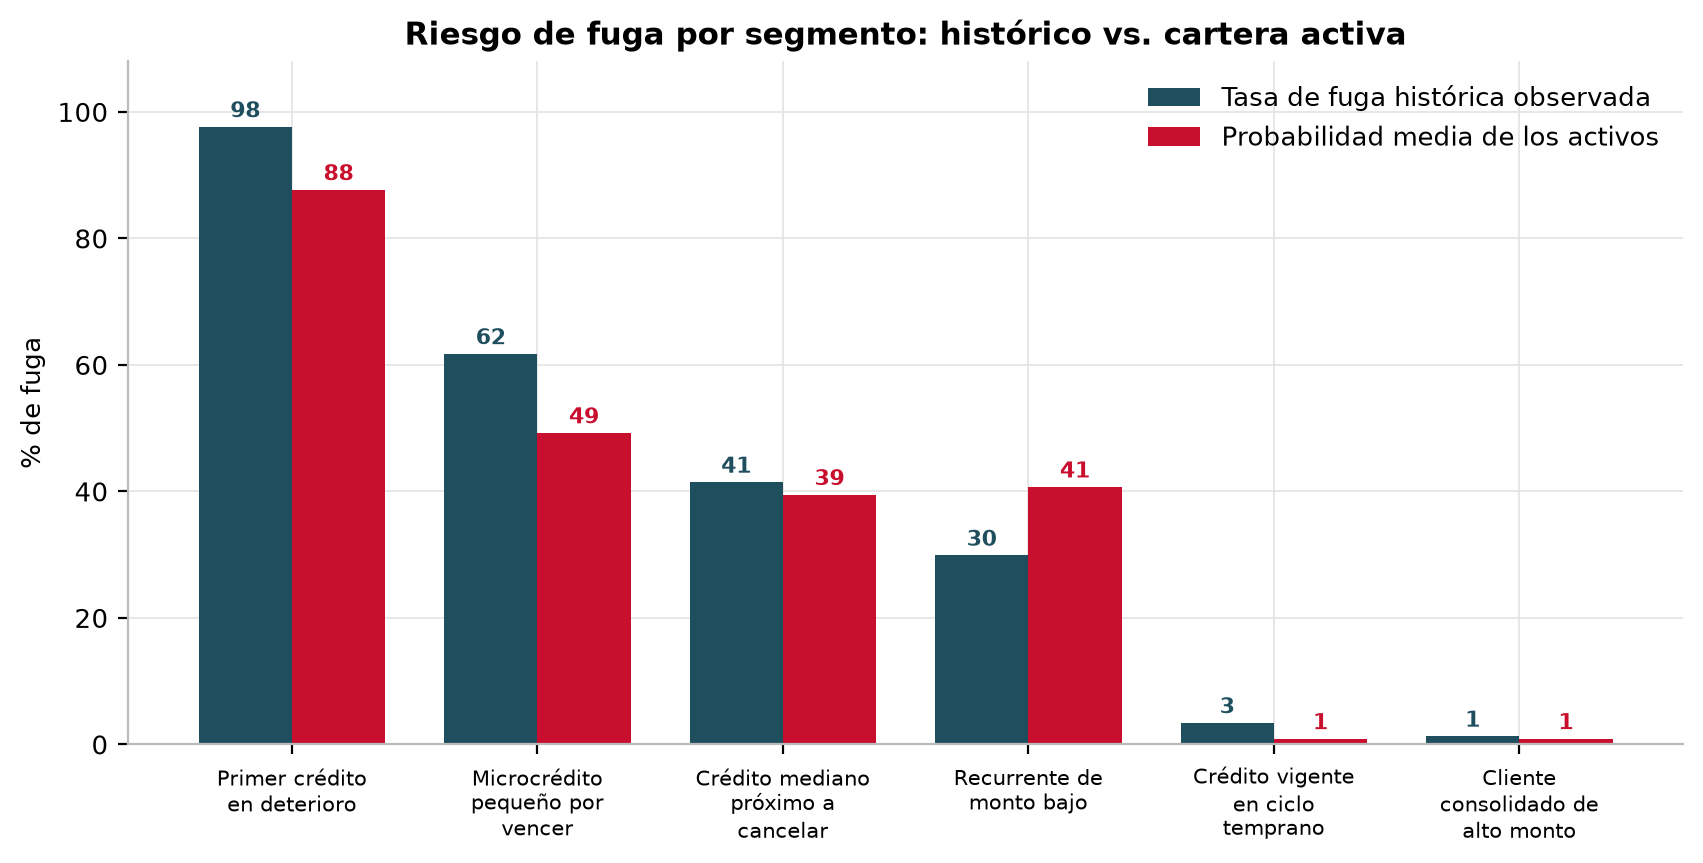
\includegraphics[width=0.86\textwidth]{outputs/figuras/08_riesgo_por_cluster.png}
\caption{Tasa de fuga histórica observada frente a probabilidad media asignada a
los clientes activos del mismo segmento. La correspondencia entre ambas es una
validación cruzada entre los dos ejercicios: el modelo de fuga y el de
segmentación, construidos por separado, coinciden.}
\end{figure}

\subsubsection*{Fichas de segmento}

\begin{description}[leftmargin=1.4em,style=nextline]
\item[Primer crédito en deterioro --- 6.3\% de clientes, 2.1\% de cartera, fuga 97.7\%]
      El 100\% está en etapa M2 o M3 y el 73\% cursa su primer crédito. Capital
      mediano de \$5\,000. \emph{Acción:} esto no es un problema comercial sino de
      cobranza y reestructuración. Gastar presupuesto de retención aquí es gastarlo
      mal; lo que corresponde es gestión de recuperación.
\item[Microcrédito pequeño por vencer --- 29.1\% de clientes, 5.2\% de cartera, fuga 61.8\%]
      El segmento más numeroso y el que más fugas aporta en volumen. Capital
      mediano de \$3\,000, tasa alta (43.6), 86\% del crédito ya pagado, dos
      créditos de trayectoria, 71\% mujeres. \emph{Acción:} oferta de renovación
      anticipada con monto escalonado, disparada automáticamente al alcanzar el
      80\% de amortización. Es el segmento donde la intervención temprana rinde más.
\item[Crédito mediano próximo a cancelar --- 15.2\% de clientes, 10.5\% de cartera, fuga 41.5\%]
      Capital mediano de \$12\,000, cuatro créditos de trayectoria, tasa baja (30),
      89\% amortizado. Son clientes buenos y recurrentes justo en el punto de
      decisión. \emph{Acción:} renovación proactiva con incremento de monto. Es
      cartera de valor que se está dejando ir.
\item[Recurrente de monto bajo --- 23.2\% de clientes, 6.5\% de cartera, fuga 29.9\%]
      Cuatro créditos, capital mediano de \$5\,000, 83\% mujeres --- la mayor
      concentración femenina de la cartera. \emph{Acción:} fidelización con
      beneficio por antigüedad y mejora de tasa.
\item[Crédito vigente en ciclo temprano --- 14.4\% de clientes, 28.3\% de cartera, fuga 3.4\%]
      Desembolso reciente, 64\% del capital pendiente. \emph{Acción:} ninguna.
      Contactarlos consumiría presupuesto sin efecto: no se están yendo.
\item[Cliente consolidado de alto monto --- 11.7\% de clientes, 47.3\% de cartera, fuga 1.3\%]
      Capital mediano de \$20\,000, seis créditos, tasa preferencial. Concentran
      casi la mitad de la cartera con la menor tasa de fuga. \emph{Acción:} gestión
      personalizada por ejecutivo de cuenta. El riesgo aquí no es la fuga
      silenciosa sino la pérdida de un cliente de alto valor por desatención.
\end{description}

\subsection{Cruce entre segmento y riesgo de fuga}

\begin{table}[H]\centering\small
\caption{Clientes activos por segmento y nivel de riesgo, con el saldo expuesto en
riesgo alto. Es la matriz que convierte dos ejercicios separados en una sola
priorización.}
\T{cruce}
\end{table}

\subsection{Patrones encontrados}

\begin{enumerate}[leftmargin=*]
\item \textbf{La fuga es un fenómeno de ventana, no de perfil.} El factor que más
      separa a quien se va de quien se queda no es su monto, su región ni su sexo:
      es en qué punto del ciclo de su crédito se encuentra. Los tres segmentos de
      mayor fuga son precisamente los que tienen el crédito casi liquidado.
\item \textbf{La antigüedad protege, y protege mucho.} La tasa de fuga cae de
      34.5\% en el segundo crédito a 4.3\% en el octavo. Cada renovación lograda
      reduce de forma marcada la probabilidad de la siguiente deserción: retener
      hoy tiene retorno compuesto.
\item \textbf{El valor y el riesgo están en extremos opuestos de la cartera.} El
      47\% del saldo está en el segmento con 1.3\% de fuga; los segmentos con fuga
      superior al 60\% suman apenas el 7\% de la cartera. Gestionar por saldo en
      riesgo llevaría a ignorar a casi todos los clientes que efectivamente se van.
\item \textbf{El monto pequeño y la tasa alta van juntos, y ambos con la fuga.}
      Los segmentos de menor capital pagan tasas de 43.6 frente al 30 de los
      segmentos consolidados. Es la estructura habitual del microcrédito, pero
      señala una palanca concreta: la tasa relativa a los pares del mismo producto
      figura entre las cinco variables más predictivas.
\item \textbf{Hay un efecto de agencia que las variables del cliente no explican.}
      La agencia aporta el 7\% del peso del modelo. Dos clientes idénticos
      atendidos en agencias distintas tienen probabilidades de retención
      apreciablemente diferentes, lo que apunta a prácticas comerciales locales
      replicables.
\end{enumerate}

%==================================================================== 6
\section{Reglas de asociación --- base Bakery}

\subsection{Reglas encontradas}
\label{sec:reglas}
\inciso{2.a}

La base contiene \NTickets\ tickets y 50 productos, con un promedio de
\ItemsTicket\ artículos por ticket. Se usó \textbf{FP-Growth} (más eficiente que
Apriori) con soporte mínimo de 1\%, umbral bajo y apropiado para tickets cortos.
Se obtuvieron 124 conjuntos frecuentes y \NReglas\ reglas con lift superior a 1.

\begin{table}[H]\centering\small
\caption{Las \NCanastas\ canastas seleccionadas, ordenadas por lift.}
\T{reglas}
\end{table}

\begin{figure}[H]\centering
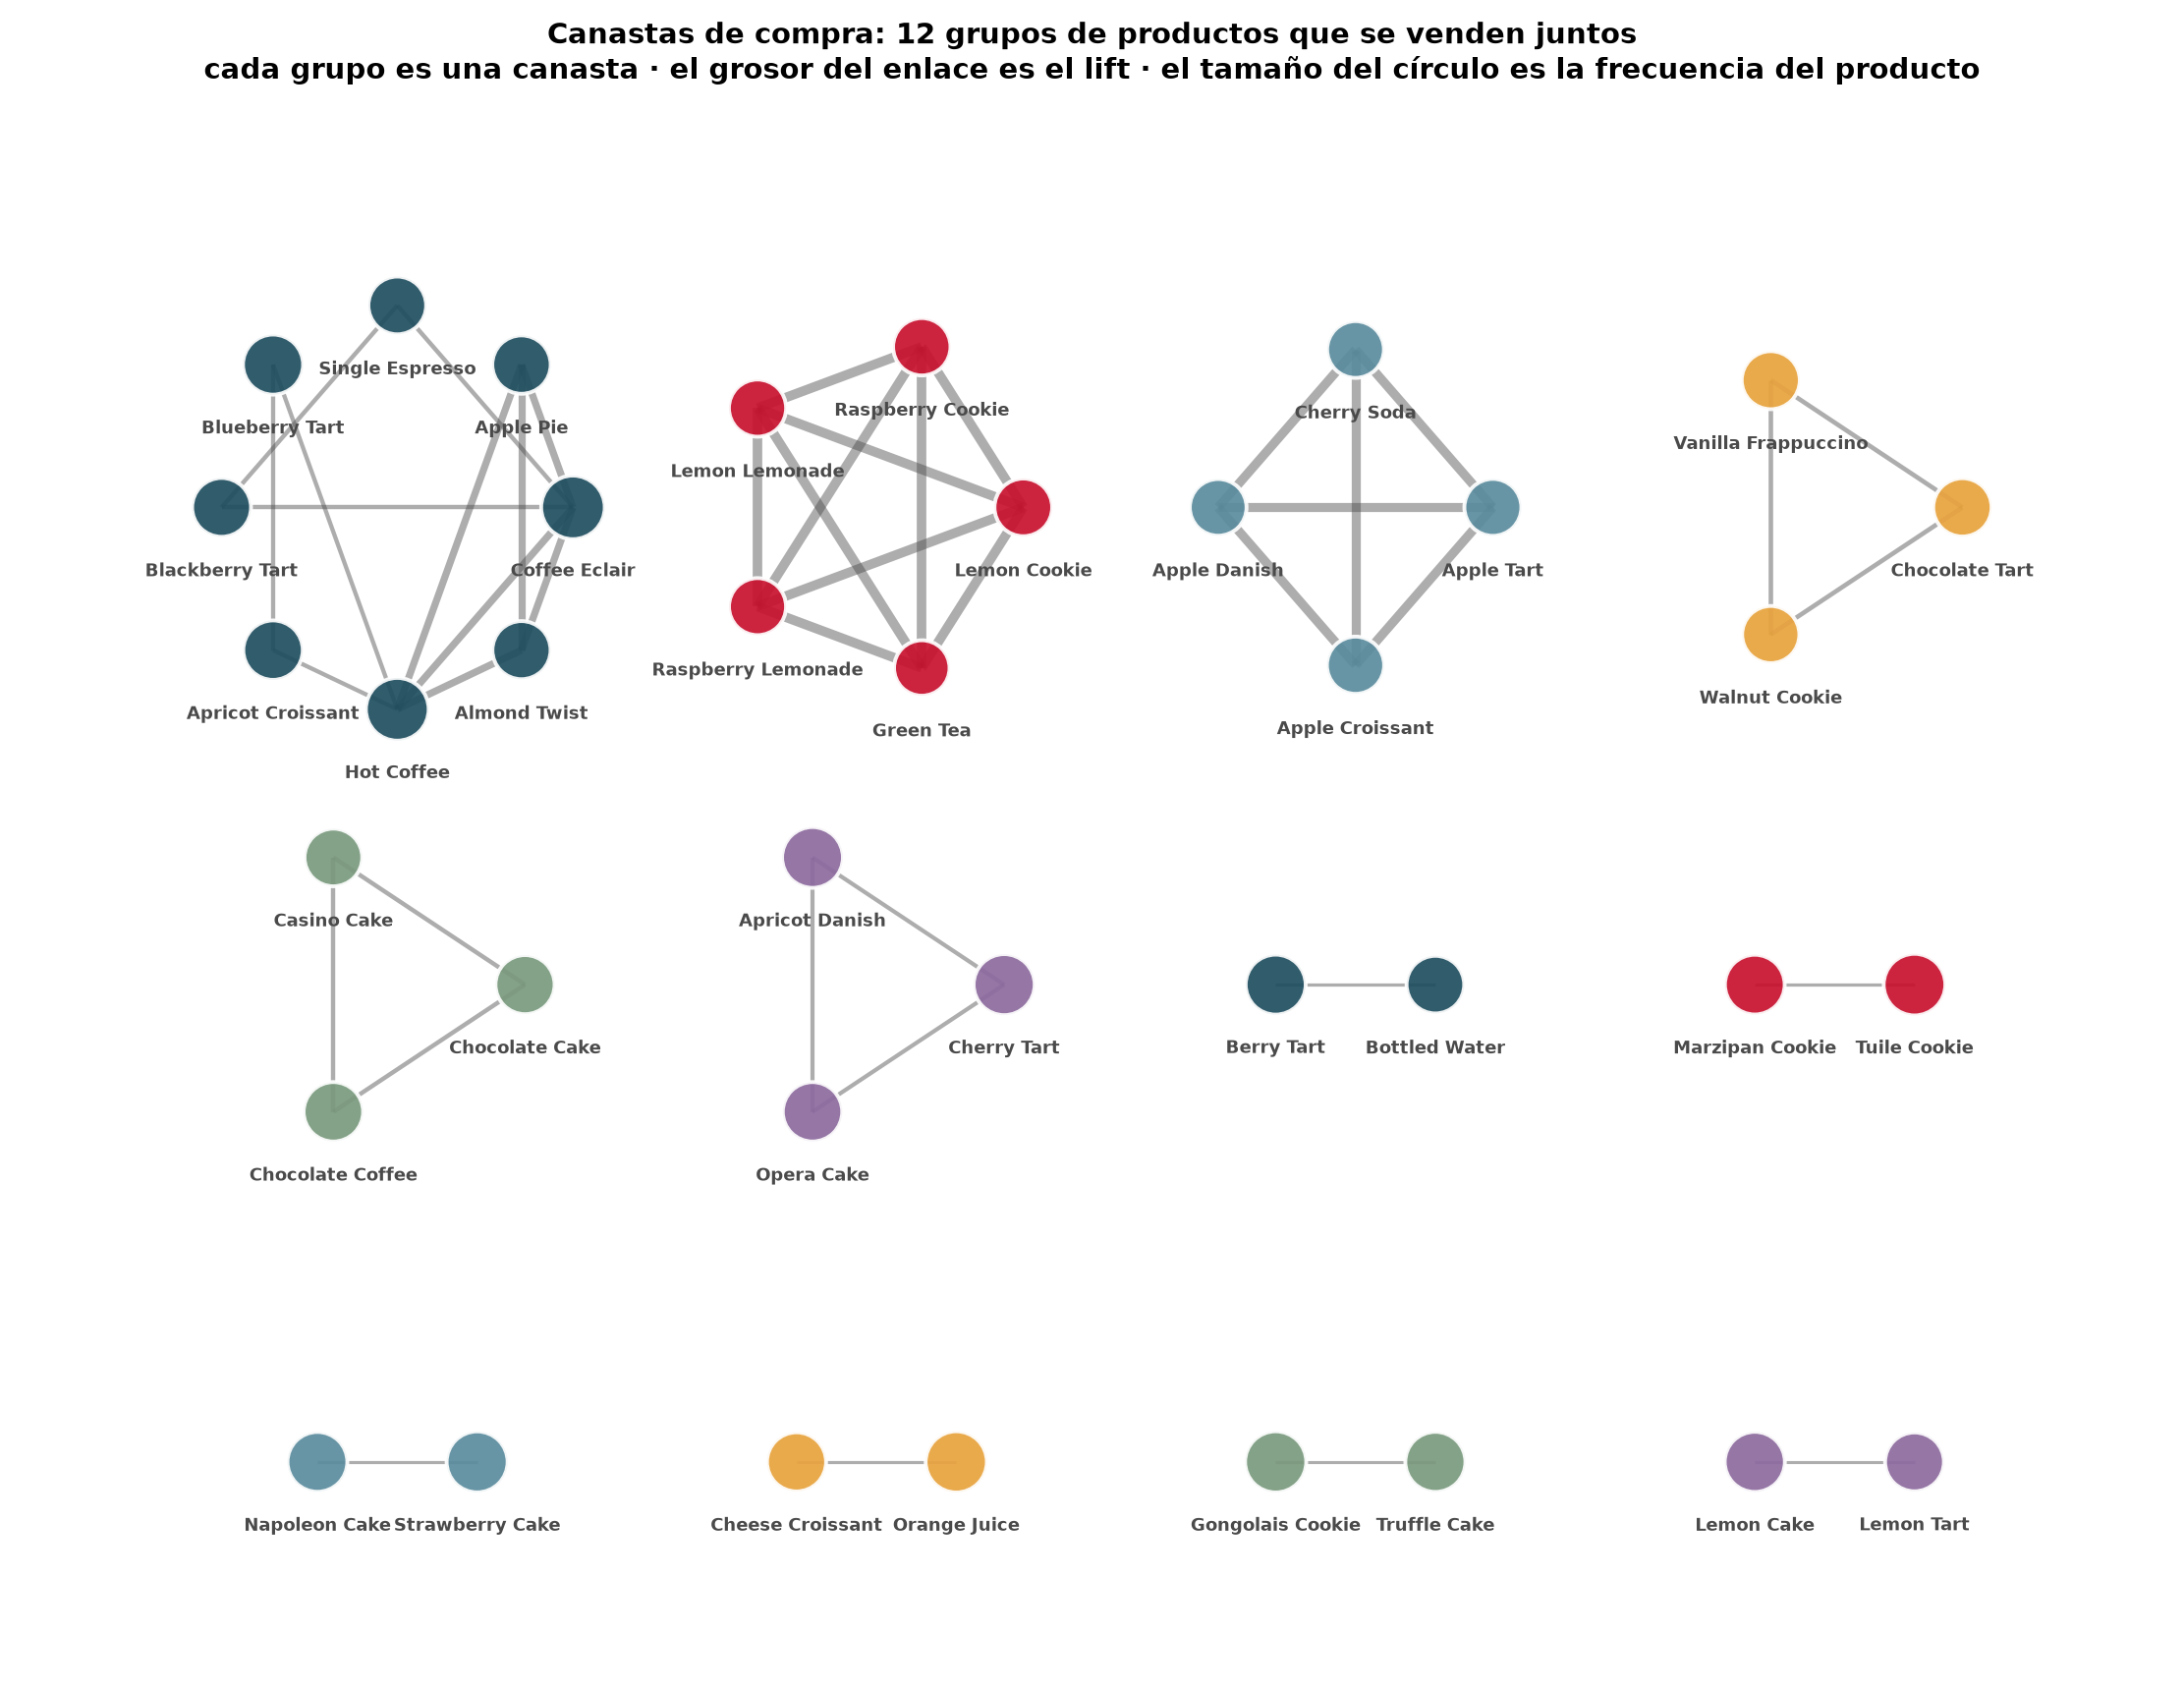
\includegraphics[width=0.9\textwidth]{outputs/figuras/09_red_productos.png}
\caption{Red de co-ocurrencia entre productos. Los conglomerados corresponden a
las canastas identificadas.}
\end{figure}

\subsection{Criterio de selección de las reglas}
\label{sec:criterio}
\inciso{2.b}

Se aplicaron cuatro filtros simultáneos y un paso de depuración:

\begin{enumerate}[leftmargin=*,nosep]
\item \textbf{Lift $> 1.20$} --- que la asociación sea real y no un efecto de la
      popularidad de los productos.
\item \textbf{Al menos 100 tickets de respaldo} --- que el hallazgo tenga
      sustento muestral y no sea una coincidencia de una veintena de compras.
\item \textbf{Confianza superior a 1.2 veces el soporte del consecuente} --- que
      la regla mejore de forma apreciable sobre la línea base de comprar ese
      producto sin más.
\item \textbf{Leverage positivo} --- co-ocurrencia por encima de lo esperado bajo
      independencia.
\end{enumerate}

\begin{alerta}[La patología de esta base no es la habitual]
El error clásico en una panadería es presentar reglas con confianza altísima y
lift cercano a 1: ``quien compra X también compra pan'' es cierto de todo el
mundo y no informa nada. \textbf{Aquí ese problema casi no existe}: el producto
más vendido, \ProdTop, aparece apenas en el \SoporteTop\% de los tickets, así que
no hay ningún artículo ubicuo que genere reglas triviales. De hecho, ninguna de
las \NReglas\ reglas tiene confianza superior al 20\% con lift inferior a 1.20.

\textbf{La patología dominante en esta base es la redundancia.} Las \NReglas\
reglas describen sólo 74 conjuntos de productos distintos, y esos 74 se reducen a
\NCanastas\ hallazgos comerciales independientes. El conjunto \{Lemon Cookie,
Raspberry Cookie, Lemon Lemonade, Raspberry Lemonade, Green Tea\} genera por sí
solo \textbf{180 reglas} con métricas casi idénticas --- todas las formas de
repartir esos cinco productos entre antecedente y consecuente --- y el conjunto de
los cuatro productos de manzana genera otras 50. Presentar ese recuento como 230
hallazgos sería un error de lectura: son dos.
\end{alerta}

\noindent El paso de depuración consistió, por tanto, en \textbf{colapsar cada
regla a su conjunto de productos subyacente} (antecedente unido a consecuente),
conservar una sola regla representante por conjunto --- la de mayor lift --- y
eliminar los conjuntos contenidos en otro que no lo mejorara. De \NReglas\ reglas
quedan \NCanastas\ canastas genuinamente distintas.

\subsection{Uso recomendado de los resultados}
\label{sec:usobakery}
\inciso{2.c}

\begin{enumerate}[leftmargin=*]
\item \textbf{Combos empaquetados con precio propio.} Las tres canastas de mayor
      lift se compran juntas entre 25 y \LiftMax~veces más de lo que ocurriría
      por azar. Merecen ser productos de catálogo con precio de paquete, no una
      sugerencia del vendedor: el combo \emph{Apple Croissant + Apple Danish +
      Apple Tart + Cherry Soda} aparece en 204 tickets con 93.6\% de confianza.
\item \textbf{Disposición física del mostrador.} Ubicar contiguos los productos
      de cada canasta y colocar la bebida asociada junto a su repostería. La
      canasta \emph{Almond Twist + Apple Pie + Coffee Eclair + Hot Coffee} indica
      que la vitrina de bollería y la barra de café no deberían estar separadas.
\item \textbf{Recomendador en punto de venta y en pedido en línea.} Cuando el
      cliente lleva tres de los cuatro productos de una canasta, sugerir el
      cuarto: la confianza en ese escenario supera el 90\%, la tasa más alta de
      conversión que se puede esperar de una sugerencia.
\item \textbf{Producción y compras conjuntas.} Los productos de una misma canasta
      deben planificarse con la misma proyección de demanda. Quebrar el inventario
      de uno arrastra la venta de los otros tres, lo que convierte un faltante
      puntual en una pérdida multiplicada.
\item \textbf{Cómo medir que funcionó.} Prueba A/B por sucursal o por semana,
      midiendo ticket promedio y unidades por ticket contra un grupo de control.
      Sin grupo de control, cualquier mejora observada se confunde con
      estacionalidad.
\end{enumerate}

\begin{nota}
\small \textbf{Limitación declarada:} la base no incluye fecha, hora, cantidad ni
precio unitario. No fue posible, por tanto, analizar patrones por franja horaria
--- que en una panadería cambian radicalmente entre el desayuno y la tarde --- ni
ordenar las reglas por impacto económico. Con esos campos, la priorización debería
hacerse por dinero y no por lift.
\end{nota}

%==================================================================== 7
\section{Tablero de visualización}
\label{sec:tablero}
\inciso{1.f (dashboard) y 3}

Se construyó un tablero interactivo de cinco páginas, entregado como un único
archivo HTML autónomo:

\begin{center}
\fbox{\parbox{0.9\textwidth}{\centering\vspace{3pt}\small
\texttt{Tablero\_Cartera\_Riesgo\_Julio\_Vicente.html}\\[2pt]
\footnotesize Se abre con doble clic en cualquier navegador. No requiere
servidor, conexión a internet ni instalación: los datos van embebidos en el
propio archivo.
\vspace{3pt}}}
\end{center}

\begin{description}[leftmargin=1.4em,style=nextline,nosep]
\item[Página 1 --- Predicción de fuga] Indicadores de cartera, curva de ganancia,
      distribución de probabilidades, tabla de calibración, variables de mayor
      impacto y escalera de modelos.
\item[Página 2 --- Segmentación] Fichas de los seis segmentos, comparación entre
      tasa histórica y probabilidad de los activos, cruce segmento $\times$ riesgo
      y desglose por región.
\item[Página 3 --- Canastas Bakery] Reglas depuradas, penetración de productos y
      recomendaciones de uso.
\item[Página 4 --- Simulador de campaña] Permite mover la efectividad supuesta, el
      costo de contacto y la capacidad del área comercial, y recalcula en el acto
      cuántos clientes conviene contactar, cuántas retenciones se esperan y cuál
      es el retorno. El cálculo se hace sobre los 10\,000 clientes reales, no
      sobre una aproximación.
\item[Página 5 --- Metodología] Trazabilidad de las decisiones: fuga de
      información detectada, diseño de validación y limitaciones.
\end{description}

\begin{nota}
\small \textbf{Sobre la herramienta.} El enunciado admite ``Power BI o cualquier
otro software que facilite la visualización''. Se optó por un tablero web
autónomo por dos razones. La primera es de \textbf{confidencialidad}: se trata de
información de clientes de una entidad financiera, y publicarla en un servicio de
alojamiento público de tableros sería inadecuado; este tablero funciona sin
enviar los datos a ningún servidor externo. La segunda es de portabilidad: se
abre en cualquier navegador sin licencia ni instalación. Los archivos XLSX
entregados están además listos para cargarse directamente en Power BI si se
prefiere reproducirlo en esa herramienta.
\end{nota}

%==================================================================== 8
\section{Limitaciones y siguientes pasos}

\subsection*{Lo que este modelo no puede hacer}

\begin{enumerate}[leftmargin=*]
\item \textbf{No mide el efecto de la campaña, sólo el riesgo.} Como se explicó en
      \S\ref{sec:campana}, identificar a quien se va no es identificar a quien se
      deja convencer. Requiere modelado de incrementalidad con grupo de control.
\item \textbf{No hay validación fuera de tiempo.} Las bases no traen fechas. El
      esquema de tres bloques disjuntos con agrupación por atributos es lo más
      cercano posible, pero no reproduce la degradación que sufre un modelo al
      aplicarse a un período posterior.
\item \textbf{Faltan las variables más predictivas del negocio.} Sin días de mora,
      historial de puntualidad, fechas de desembolso ni montos de créditos
      anteriores, no se pudieron construir variables de tendencia --- deterioro
      reciente frente al propio historial del cliente, caída del monto solicitado
      --- que en cartera de microcrédito suelen dominar. Incorporarlas es la
      mejora de mayor retorno disponible.
\item \textbf{La deriva entre bases es real y hay que vigilarla.} El PSI de 2.74
      en capital concedido indica que las dos poblaciones no son idénticas. El
      diseño lo mitiga apoyándose en ratios, pero conviene recalcular el PSI en
      cada aplicación del modelo.
\item \textbf{El segmento de primer crédito descansa en un supuesto explícito.}
      La tasa de \TasaKuno\% proviene de extrapolar la curva de fuga, no de
      observación directa. Es la estimación defendible con los datos disponibles,
      y su sensibilidad está cuantificada, pero sigue siendo un supuesto.
\end{enumerate}

\subsection*{Plan sugerido}

\begin{enumerate}[leftmargin=*,nosep]
\item Ejecutar la primera campaña con 10\% de grupo de control aleatorio.
\item Incorporar variables de comportamiento de pago y fechas al conjunto de
      entrenamiento; reentrenar y comparar contra la línea base actual.
\item Monitorear mensualmente el PSI de las variables de entrada y la calibración
      observada por decil. Reentrenar cuando la calibración se desvíe.
\item Con los resultados de la campaña con control, entrenar un modelo de
      incrementalidad para el segundo ciclo.
\end{enumerate}

%==================================================================== ANEXOS
\appendix
\clearpage
\section{Evidencia de la auditoría de datos}
\label{ap:evidencia}

Detalle numérico de las tres condiciones de los datos enunciadas en
\S\ref{sec:datos}.

\subsection*{Las dos fugas de información}

\begin{alerta}[Hallazgo 1 --- los identificadores contienen la respuesta (AUC = 1.000)]
Todos los clientes retirados tienen código entre 1 y 34\,354, y todos los
renovados entre 34\,355 y 88\,828: rangos \textbf{disjuntos}. La regla
``código $\leq$ 34\,354 $\Rightarrow$ retirado'' acierta en el 100.0000\% de los
78\,829 registros. El código no describe al cliente, describe el orden en que se
ordenó el archivo antes de numerarlo --- y en la base de predicción los códigos
fueron renumerados de 1 a 10\,000, donde no contienen señal alguna. Ambas
columnas se descartaron.
\end{alerta}

\begin{alerta}[Hallazgo 2 --- el primer crédito es el objetivo escrito de otra forma]
Los 12\,791 clientes históricos con \texttt{CREDITOS ANTERIORES} igual a 1 son
retirados \emph{sin una sola excepción}. No es una tasa alta: es una identidad
lógica, porque renovar exige por definición un segundo crédito. En la base de
predicción hay 1\,873 activos en esa situación (18.7\%): su desenlace todavía no
ha ocurrido y asignarles 100\% de probabilidad sería trasladar la tautología. El
tratamiento se describe en \S\ref{sec:primercredito}.
\end{alerta}

\subsection*{Deriva de montos entre las dos bases}

El capital concedido presenta un PSI de 2.74, muy por encima del umbral de 0.25
que indica inestabilidad, por una causa estructural: las bases usan rejillas de
montos casi disjuntas. Los valores \$3\,000, \$4\,000 y \$15\,000, que cubren el
30\% del histórico, están prácticamente ausentes entre los activos; a la inversa,
\$5\,000 concentra el 42.6\% de los activos y apenas el 7.6\% del histórico. La
respuesta de diseño fue apoyar el modelo en el ratio saldo/capital, invariante a
la escala del monto.

\subsection*{El saldo sí es comparable entre bases}

Se verificó que la distribución del ratio saldo/capital en los activos se sitúa
\emph{entre} la de renovados y la de retirados, con distancia de
Kolmogorov--Smirnov de 0.144 contra el histórico completo, frente a 0.31 y 0.39
contra cada clase por separado. Si el saldo del histórico se hubiera medido
después del desenlace, los activos se parecerían a los renovados; no es el caso.

\clearpage
\section{Reproducibilidad}

Todo el análisis es reproducible ejecutando en orden los guiones de la carpeta
\texttt{src/}. Semilla fija (42) en particiones, modelos y remuestreos.

\begin{description}[leftmargin=1.4em,style=nextline,nosep]
\item[\texttt{00\_reconocimiento.py}] Estructura, esquemas y compatibilidad entre bases.
\item[\texttt{01\_auditoria.py}] AUC univariado, deriva, calidad, duplicados.
\item[\texttt{02\_auditoria\_fina.py}] Hojas adicionales, deriva de montos, forma de las relaciones.
\item[\texttt{03\_trampa\_identificadores.py}] Confirmación forense de las dos fugas de información.
\item[\texttt{04\_comparabilidad.py}] Verificación de que el saldo es comparable entre bases.
\item[\texttt{features.py}] Limpieza e ingeniería de variables compartida.
\item[\texttt{05\_modelado.py}] Escalera de modelos, validación, calibración, modelo final.
\item[\texttt{06\_shap.py}] Importancia SHAP, contraste con la logística, estabilidad.
\item[\texttt{07\_prediccion.py}] Probabilidades de los 10\,000, deciles, valor esperado.
\item[\texttt{08\_clustering.py}] Segmentación, elección de $k$, estabilidad, perfilado.
\item[\texttt{09\_bakery.py}] Reglas de asociación y depuración.
\item[\texttt{10\_entregables.py}] Construcción de los archivos XLSX.
\item[\texttt{11--13}] Datos del tablero, tablero y tablas del informe.
\end{description}

\subsection*{Hiperparámetros del modelo final}

LightGBM: objetivo binario, 700 árboles, tasa de aprendizaje 0.05, 48 hojas,
mínimo 60 observaciones por hoja, submuestreo 0.85, submuestreo de columnas 0.80,
regularización L1 0.5 y L2 2.0, semilla 42. Categóricas tratadas de forma nativa.
Calibración: regresión isotónica con recorte fuera de rango.

\subsection*{Entorno}

Python 3.12.7; pandas 3.0.5, numpy 2.5.2, scikit-learn 1.9.0, LightGBM 4.7.0,
SHAP 0.52.0, mlxtend 0.25.0. Versiones exactas en \texttt{requirements.txt}.

\end{document}
